
%%%%%%%%%%%%%%%%%%%%%%%%%%%%%%%%%%%%%%%%
%          Leg Mechanical Design
%%%%%%%%%%%%%%%%%%%%%%%%%%%%%%%%%%%%%%%%

\section{Mechanical Design of The Leg}
\label{sec:LegDesign}

With actuator from $\color{red}section$ and linkage design from $\color{red}section$, this section presents a detailed mechanical design layout of the leg. The leg module is composed of three motor modules(HIP/KNEE/ABAD), each has a motor coil and a planetary gearbox with moderate gear ratio to achieve the Quasi-Direct-Drive\cite{20162016} strategy. To accommodate size limitation imposed by actuator choice, the two-stage compound planetary gearbox is used as the transmission. The leg is design to optimize for large workspace, with the novel HIP-KNEE connection design, the knee joint could rotate $360^{\circ}$, the curved upper link and hollow thigh link design also enables large knee joint workspace.
  
\begin{figure}
	\centering
	\resizebox{1\linewidth}{!}{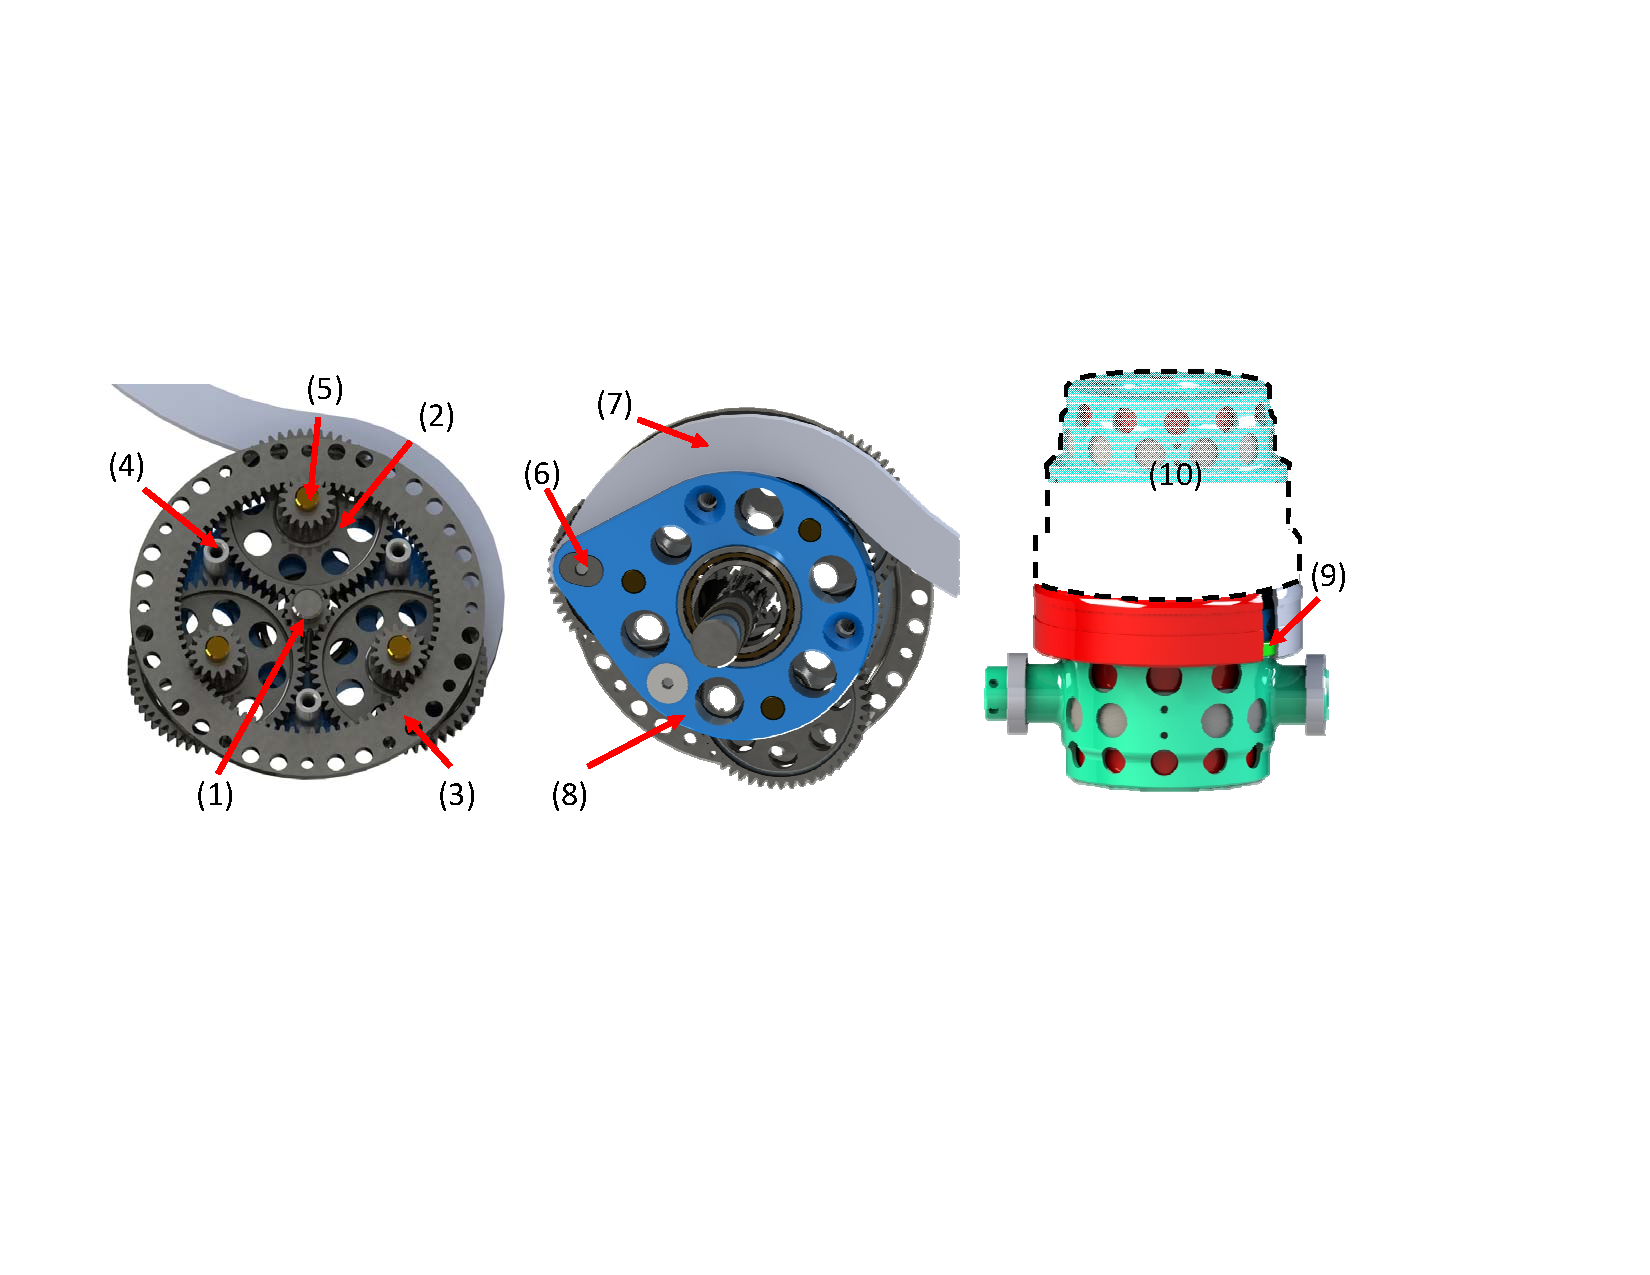
\includegraphics{gearbox.pdf}}
	\caption{Planetary gearbox design with three compound planet gears (left); curved upper-link design (middle); hip and knee motor module (right); (1) sun gear, (2) compound planet gear, (3) ring gear, (4) stand-off, (5) brass dowel pin, (6) output pin, (7) upper link, (8) KNEE carrier, (9) KMF PBXS020 bearing, (10) the KNEE motor module}
	\label{fig:gearbox}
\end{figure}



\subsection{HIP-KNEE Connection Design}
\label{sec:Design4ROM}

\begin{figure}
	\centering
	\resizebox{1.0\linewidth}{!}{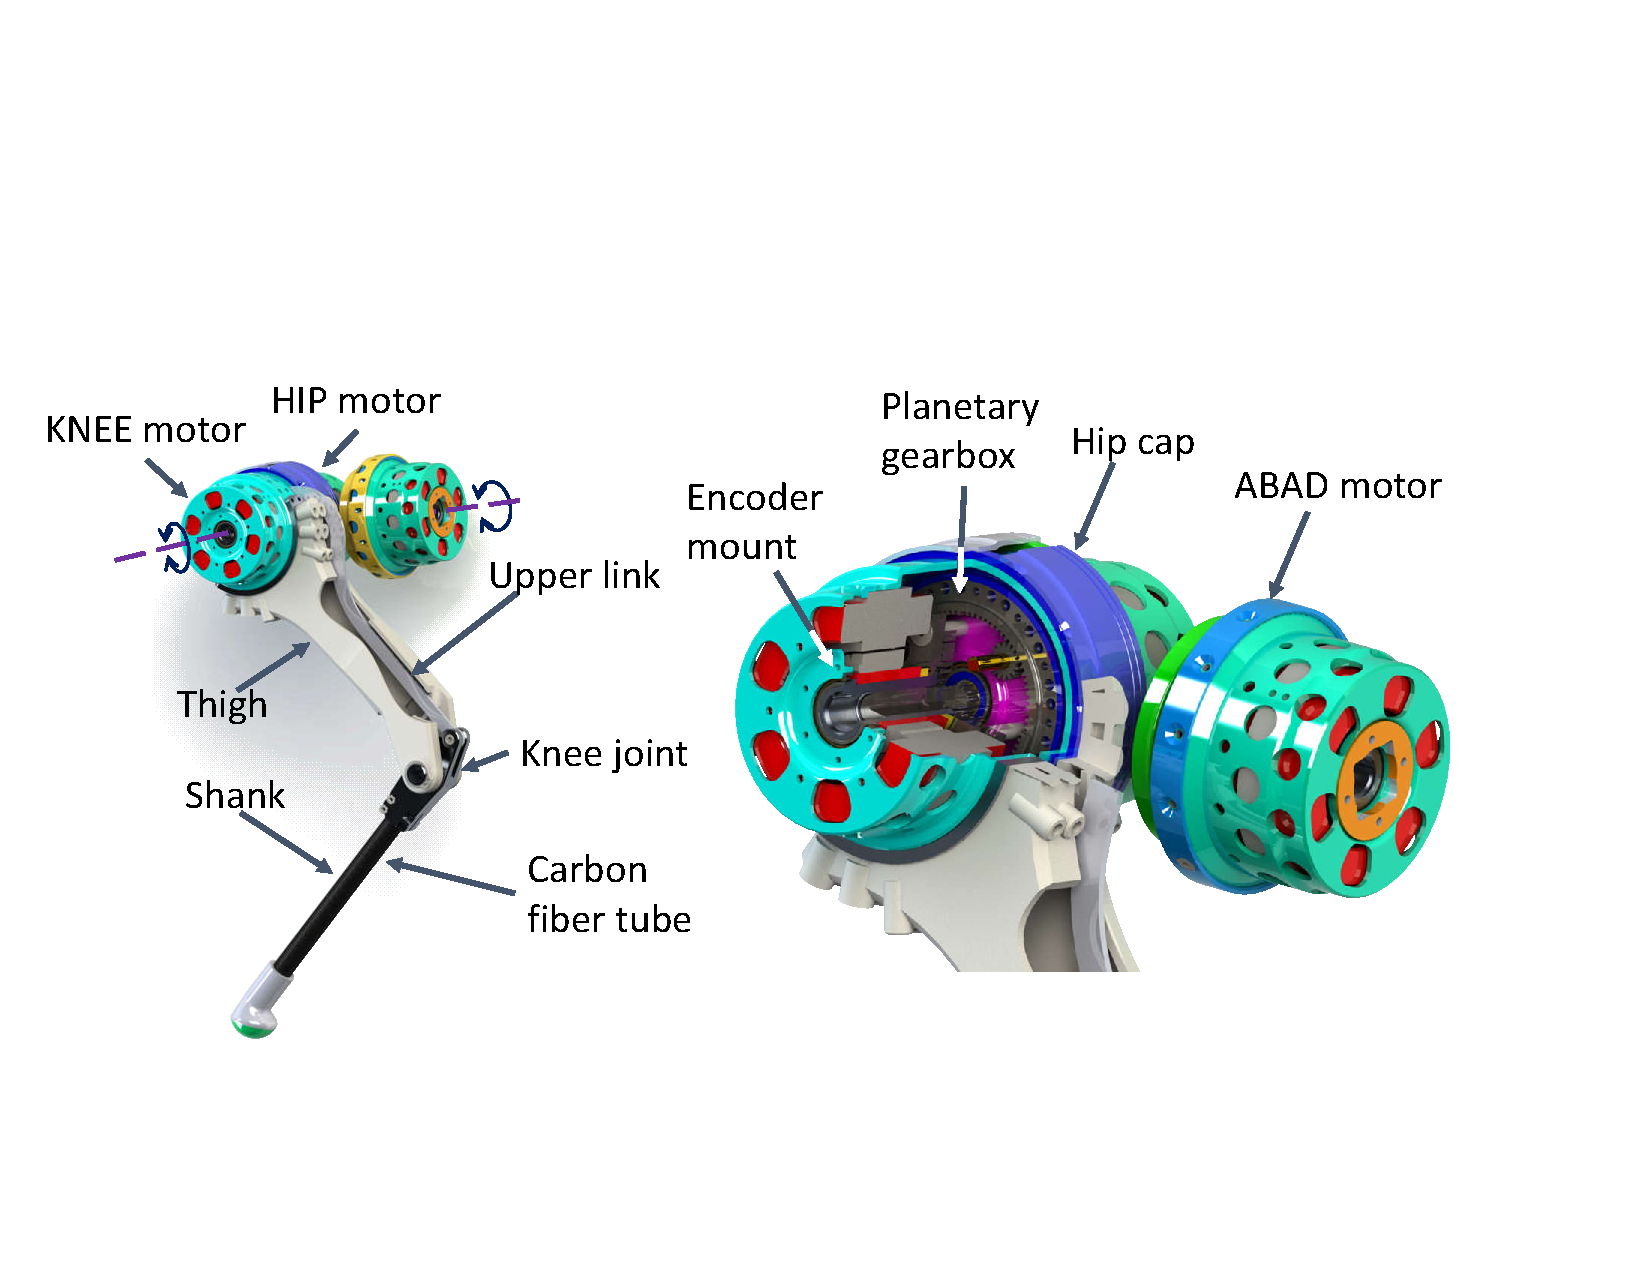
\includegraphics{SWrendering.pdf}}
	\caption{CAD Model of the Leg Module Design; (left) A side-view of the leg module with cut-out on thigh link showing the four-bar linkage design; (right) A cut-out view showing the internal structure of a motor module}
	\label{fig:LegDesign}
\end{figure}
\begin{figure}
	\centering
	\resizebox{1.0\linewidth}{!}{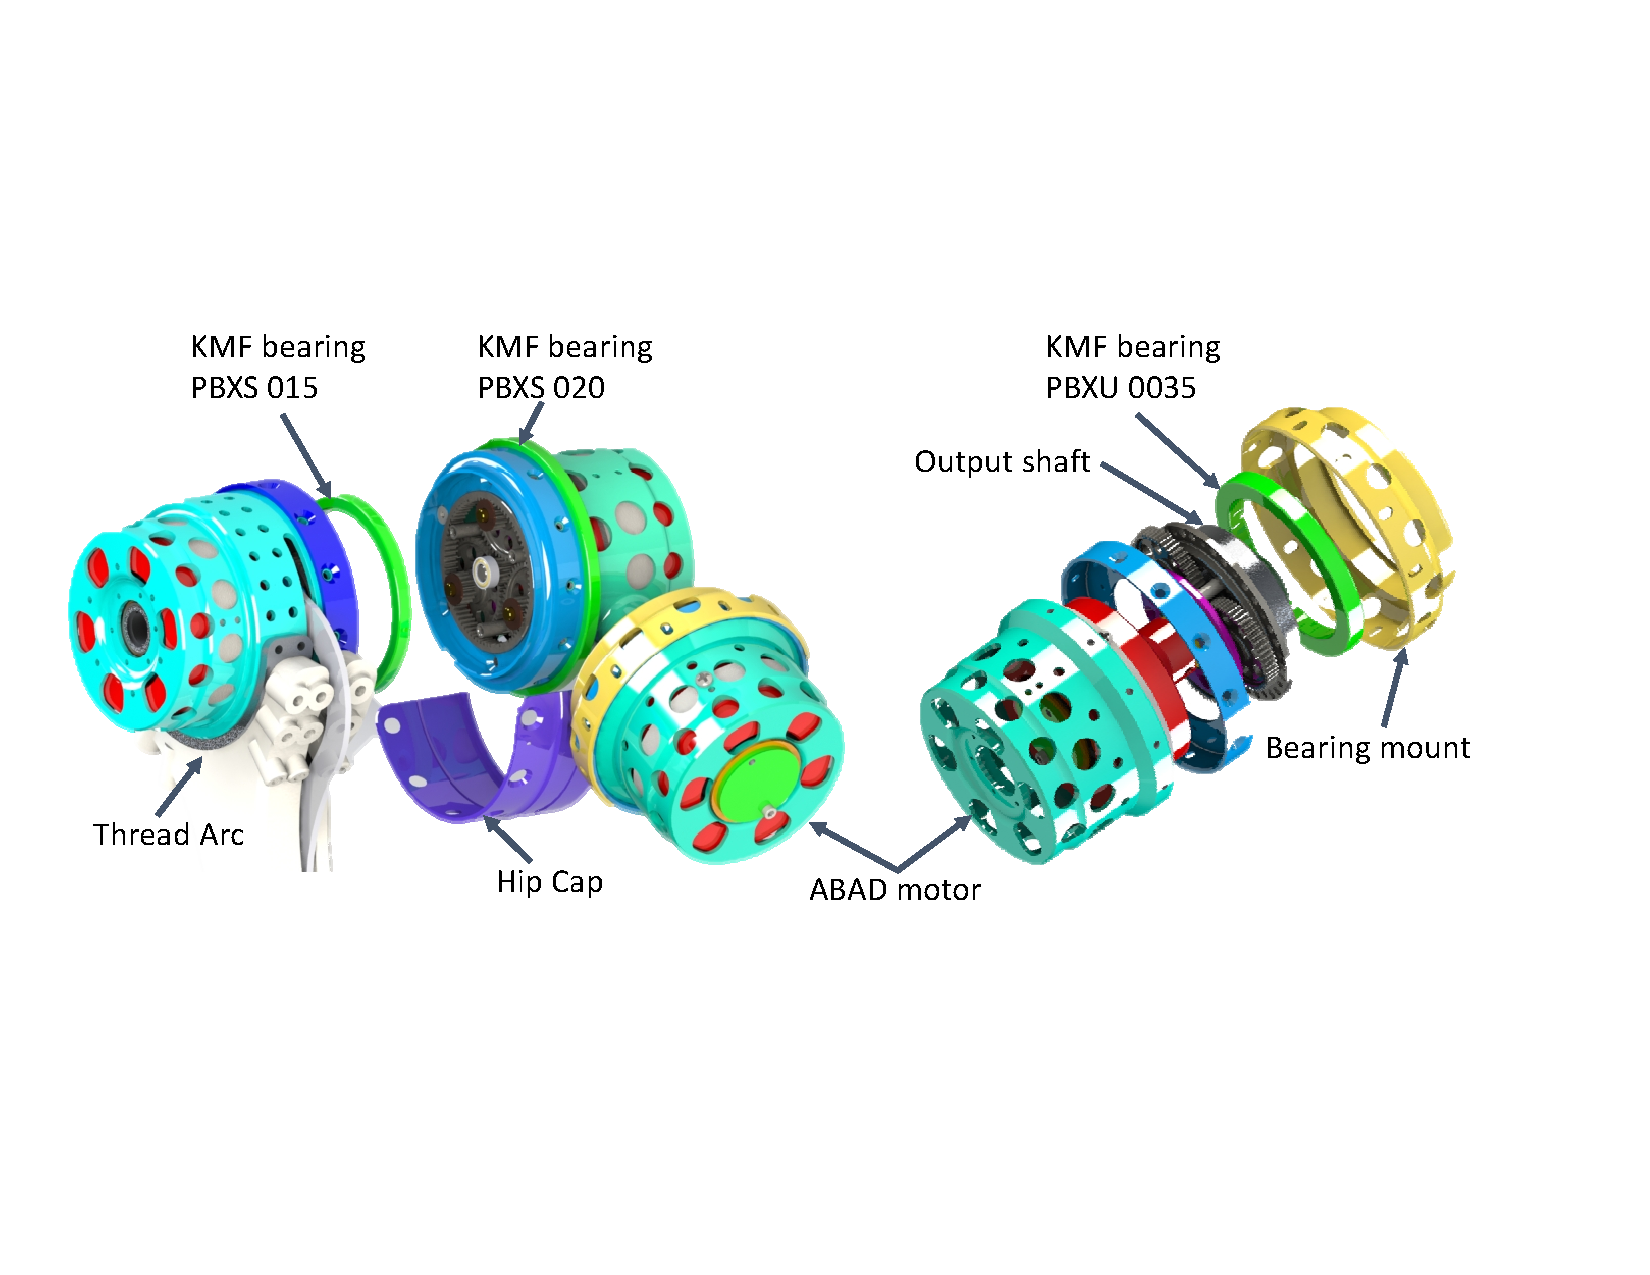
\includegraphics{KMFbearings.pdf}}
	\caption{(left) Connection Design Between HIP and KNEE Motors for Large Hip Range of Motion (ROM); (right) Exploded View of ABAD motor}
	\label{fig:KMFbearings}
\end{figure}

Each leg module is composed of three brush-less DC (BLDC) motor modules. HIP, KNEE, ABAD stand for hip joint, knee joint and abduction/adduction joints respectively. The HIP and KNEE motors are placed face-to-face and coaxially as shown in Figure \ref{fig:LegDesign}. Double supported by two thin-section bearings (KMF: PBXS020/ PBXS015), the KNEE motor could rotate $360^{\circ}$ with respect to the HIP motor. One bearing (KMF: PBXS015) is located between HIP and KNEE motors and the other one (PBXS020) is located outside of the HIP motor shell and enclosed by two hip caps. An explosive view could be found in Figure \ref{fig:KMFbearings}. The HIP motor shell's outer surface is used as one of bearing PBXS020's mating surface, and the inner surface of the Hip cap is used as the other mating surface. The hip cap is fixed to the KNEE motor and grips on the HIP motor via PBXS020 bearing, allowing the KNEE motor to rotate freely related to the HIP motor.

The ABAD motor's rotational axis is placed perpendicular to the HIP/KNEE motors' axis. The internal structure of the ABAD motor is shown in Figure \ref{fig:KMFbearings}. The torque produced by electrical coil is magnified by the planetary gearbox and transfered to the output shaft, whose motion is constrained by the bearing mount via another thin-section bearing(KMF PBXU0035). The output shaft of ABAD motor is directly connected to the HIP/KNEE module. With transmission eliminated, the workspace of the ABAD joint is not limited by the leg itself. 

\subsection{\textbf{Linkage Transmission Design}}
\label{sec:legDesign}

The linkage transmission design is shown in Figure \ref{fig:LegDesign}. The torque of the KNEE motor is transmitted to the knee joint through a four-bar linkage mechanism. Hence the KNEE motor could be put nearer to the main body and the rotary inertia could be reduced. The 3D printed hollow thigh design allows the curved upper link to travel inside without interference, while providing protection to the upper link. Consequently, the robot-human interface would be safer. In addition, the curved upper link design allows larger knee joint workspace compared with straight link design As shown in Figure \ref{fig:gearbox}, the curved link avoids the standoff (4) in the figure and gains $27^{\circ}$ more rotation angle compared with straight four-bar linkage design.

The thigh link was connected to the KNEE motor surface through four screws initially. During preliminary jumping tests it turned out that the large ground impact impulse at touch down would rip off the thread on the KNEE motor shell. To solve this problem, an additional part called thread arc was made to provide more threaded holes on the knee motor. Figure \ref{fig:KMFbearings} shows that the thread arc is attached to the KNEE motor surface and the new thigh link is fixed to the thread arc with 18 screws to evenly distribute the load.

\subsection{\textbf{Electronic System Integration}}
\label{sec:Electronics}

The electronic system of the robot leg consists of the following components: two Elmo Gold Twitter amplifiers were used for motor commutation, two RLS-RMB20 magnetic encoders were used to measure motor angle, ATI Mini40 F/T sensor was used to measure the ground reaction force created by the leg. The control loop runs at 4kHz on an Intel i5 desktop in Simulink Real-Time. 


